\documentclass[12pt]{article}
\usepackage[sort&compress,numbers,super]{natbib}
\usepackage{charter,fancyhdr,wrapfig,color,lastpage}
\usepackage{setspace}
\onehalfspacing
\usepackage{float}
\usepackage[toc,page]{appendix}
\usepackage{amsmath,amssymb,amstext}
\usepackage{enumerate}
\usepackage{graphicx}          
\usepackage{tabularx}
\usepackage{siunitx}
\usepackage[version=4]{mhchem}
\usepackage{chemmacros}
\chemsetup{
	modules = all,
	formula = mhchem
}

\definecolor{Red}{rgb}{0.8,0.2,0.2}
\definecolor{Blue}{rgb}{0.2,0.2,0.8}

\sloppy
\textwidth=6.5in \textheight 9in \oddsidemargin=0in \topmargin=-0.5in

\cfoot{\thepage}

\begin{document}

\begin{center}
\section*{Title of your Thesis}

A Thesis\\
Presented to\\
The Faculty of the Department of Chemistry and Biochemistry\\
Bates College\\
in partial fulfillment of the requirements for the\\
Degree of Bachelor of Science\\
\vspace{5mm}
By\\
Your Name\\
Lewiston, ME\\
Thesis date\\

\end{center}

\clearpage

\begin{center}
	\textbf{Acknowledgments}\\
\end{center}

Write acknowledgments here.

\clearpage


\begin{center}
	Write dedication here.
\end{center}

\clearpage

\tableofcontents

\clearpage

\listoffigures

\listoftables

\clearpage

\begin{center}
\subsection*{Abstract}
\end{center}
\noindent
The Abstract should provide a brief introduction to your research, a brief explanation of the techniques used, any important results, and the overall impact of your work. The Abstract should be limited to one paragraph under 300 words.

\pagebreak

\section{Introduction}

The introduction section should provide the background of your research topic and highlight the relevance of your work. For example, if you were studying a particular structure type for a particular technological application, the introduction should include a description of the structure type, a description of the technological application, and the previous work that has led to the scientific problem you are addressing (\textit{i.e.} work that suggests this structure type is a promising candidate for the technological application.) If your thesis focuses heavily on one type of technique (\textit{i. e.} diffraction), give a brief introduction to the technique and what it can tell us about the materials you are studying. Your annotated bibliography is a good place to start thinking about the background of your research and the techniques you have employed. The last paragraph of the introduction should set the stage for your thesis: what is the question you are trying to answer? What is the approach you are using? What was you initial hypothesis? Don't just provide a list of answers for these questions, but use these questions to frame this paragraph. You may have several questions, which will be restated in separate sections in the discussion and results. The introduction should be approximately 15--20 pages long. \\ 

\textbf{Some basic latex commands for formatting your thesis:}\\

This is how you cite a reference.\cite{RN3864} Note the citation follows the punctuation. Avoid bunching all of your citations at the end of the sentence; rather, put the citation directly behind the relevant wording. an example of this is provided in the last paragraph of the "Experimental Methods" section. You may need to run the ``Bibliography" tool and compile a few times before your references appear.\\

If you need to insert an equation, such as the following Equation \ref{eq:1}, a great resource for LaTeX formatting of equations is HostMath (http://www.hostmath.com/).

\begin{equation} \label{eq:1}
\sum_{i=0}^{\infty} a_i x^i
\end{equation}

\vspace{5mm}
This is how you insert a figure into LaTeX, Figure \ref{Example_Fig}.

\begin{figure}[H]
	\centering 
	\includegraphics[width=5.5in]{Example_Figure} 
	\caption{Figure caption should be descriptive. Explain what the figure is showing and a basic take away message. For example: The unit cells of (a) perovskite PbTiO$_3$, (b) hexagonal YMnO$_3$, (c) illmenite NaSbO$_3$, and (d) pyrochlore AgSbO$_3$ illustrates that materials with the general chemical formula \textit{AB}O$_3$ do not necessarily have the same crystal structure.}
	\label{Example_Fig}
\end{figure}

Here is an example of a schematic diagram of an instrument, Figure \ref{Example_Instrument_Schematic}, if you wish to include one.

\begin{figure}[H]
	\centering 
	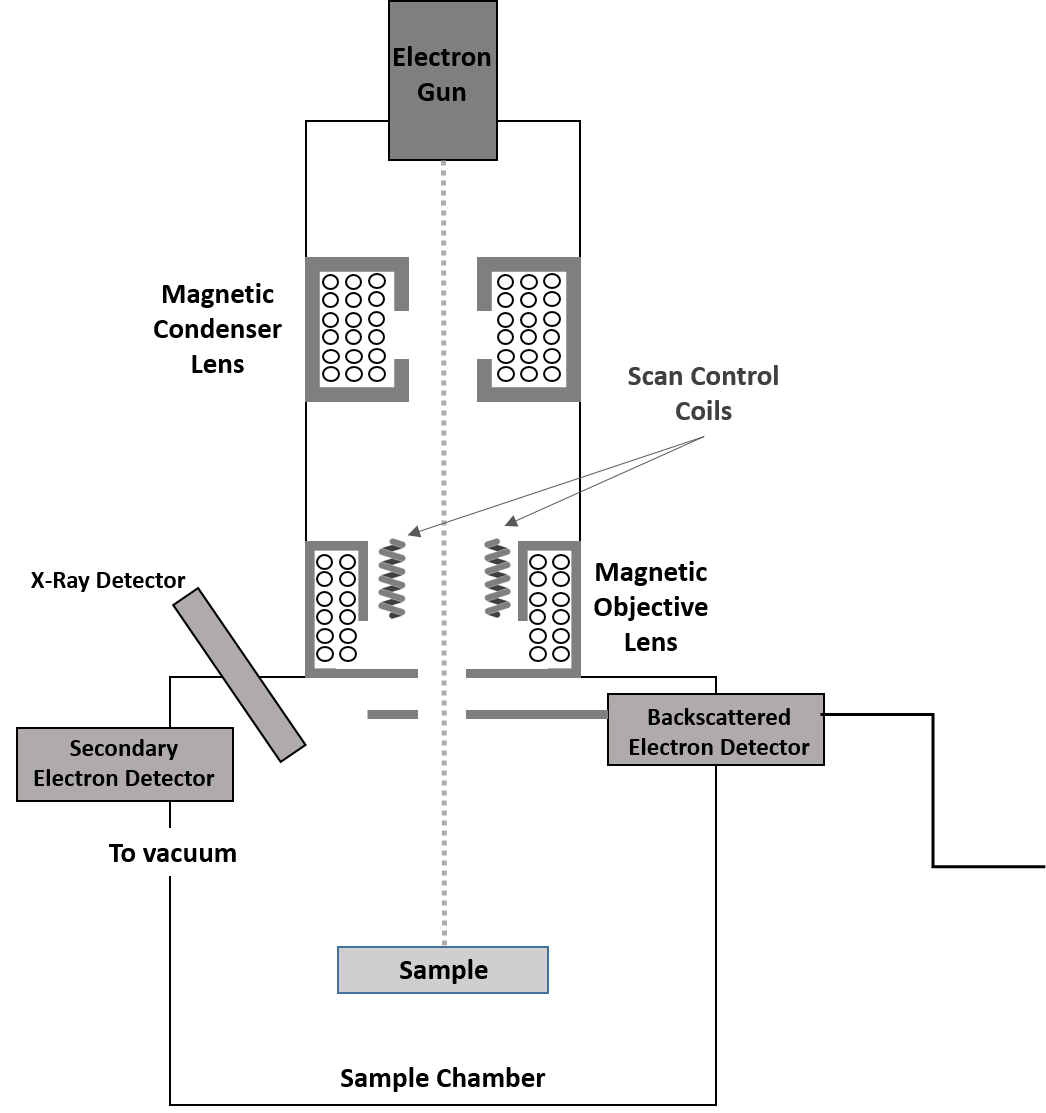
\includegraphics[width=6in]{Example_Instrument_Schematic} 
	\caption{Schematic diagram of the components of a scanning electron microscope (SEM).}
	\label{Example_Instrument_Schematic}
\end{figure}

Here is an example of how to format a table, \ref{Example_Table}:

\begin{table}[H]
	\centering
	\caption{Peak maximum and FWHM of the emission spectra. Increasing aluminum content shows a small redshift (shift towards lower energy) in the emission.}
	\label{Example_Table} 
	\begin{tabular}{llllllll}
		\hline
		\hline
		Al content $x$  & maximum (nm) & FWHM (nm)   \\
		\hline
		0.050  & 531      & 46          \\ 
		0.075 & 535      & 46          \\ 
		0.125 & 537      & 48          \\ 
		\hline
		\hline
	\end{tabular}
\end{table}

Make sure all chemical formulas and charges are properly formatted, for example: In the material Ag$_2$Sb$_2$O$_7$, the charges on the atoms are Ag$^+$, Sb$^{5+}$, and O$^{2-}$.

Make sure symbols are properly formatting, for example, the beta symbol $\beta$ and the degree symbol $^{\circ}$.

This is how you insert a chemical equation, Chemical Equation \ce{AgSbO3}:

\begin{reactions}
	AgO +Sb2O5 &->[900\,K] AgSbO3
\end{reactions}

A few other good practices for writing elegantly formatted documents include using an unbroken space between numbers and units, for example 10\,h, and italicizing all variables, for example \textit{x} in Ti$_{1-x}$Zr$_x$O$_2$.

%This is how you comment something out so that it will not be considered when you are compiling your document. It can useful if trying to find an error when compiling!

\section{Results and Discussion}

The results and discussion section should begin by reiterating the scientific problem you are investigating and your approach for investigation. This section should give a description of the techniques used to answer the scientific questions, detailed results of your research, and a discussion of meaning behind your results. Be sure to discuss all experiments that were performed, even if the experiment yielded undesirable results. Where possible, hypothesize why the experiment didn't work as planned, excluding human error! figures for this section should include illustrative examples of your results; you do not need to put every XRD pattern in this section. If you wish to include several patterns or large tables of crystallographic data, use an appendix section at the end of this document. This may be split into several sections if multiple topics were addressed. 

\subsection{Topic 1 Title}

\subsection{Topic 2 Title}

\section{Conclusions and Future Work}

The Conclusion should summarize your work, without being a direct repetition of the Abstract. This section should focus more on the broader impacts and the future directions of your work. This section should be limited to three paragraphs under 500 words each. 

\section{Experimental Methods}

The experimental methods section should provide a comprehensive explanation of your methods and experimental procedures. When writing this section, think to your self, what would I need to tell someone who was trying to reproduce my work exactly? This section should include details for samples preparation and any experimental details, including references for all software used to complete your research. All procedures that are ``standard" should be appropriately referenced. A brief example is shown below:\\

\noindent 
Polycrystalline samples of Cd$_2$Nb$_2$O$_{7-x}$S$x$ ($x$ = 0, 0.25, 0.5, and 0.7) were prepared by mixing a stoichiometric ratio of CdO (Alfa Aesar, 99.99\%), CdS (Strem Chemicals, 99.995\%), and Nb$_2$O$_5$ (Fischer Scientific, 99.999\%). Cd$_2$Nb$_2$O$_7$ was fired in air at 500\,$^{\circ}$C for 10\, h and 1000\,$^{\circ}$C for 120\,h to prevent the volatilization of Cd. Samples containing S were sealed in evacuated fused silica ampoules and annealed at 1050\,$^{\circ}$C for 24\,h. Synchrotron diffraction studies were performed with a $\lambda$ = 0.4137810 on the 11BM beam line at the Advanced Photon Source, Argonne National Laboratory. Diffraction data was refined through the Le Bail method\cite{LeBail2005} using the GSAS software and EXPGUI user interface.\cite{Larson1994,Toby2001} Crystal structures were visualized using the VESTA suite of programs.\cite{Momma2011}

\pagebreak

\appendix
\section{\\Title of Appendix A}
% the \\ insures the section title is centered below the phrase: AppendixA

Text of Appendix A is Here

\section{\\Title of Appendix B}
% the \\ insures the section title is centered below the phrase: Appendix B

Text of Appendix B is Here

\pagebreak

\addcontentsline{toc}{section}{References}
\bibliographystyle{achemso}
\bibliography{Example-bibtex}


\end{document}